\documentclass[tikz]{standalone}

\usetikzlibrary{calc,positioning,shapes,positioning,intersections,quotes,decorations.markings}
\usepackage{amsfonts,amsmath,amsthm,amssymb,mathtools,stmaryrd,mathrsfs}

\begin{document}
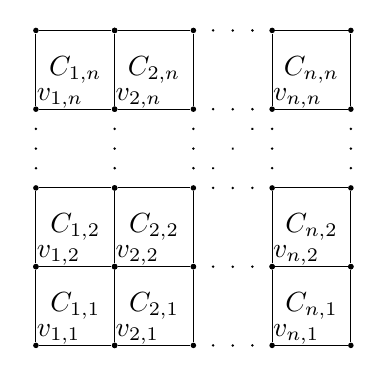
\begin{tikzpicture}[>=stealth]

	\tikzset{dotted pattern/.style={
				postaction=decorate,
				decoration={
						markings,
						mark=
						between positions 0.25 and 0.75 step 0.25
						with
							{
								\fill[radius=0.5pt,black] (0,0) circle;
							}
					}
			}
	}

	\foreach \x/\y/\nx/\ny in {0/0/1/1, 1/1/2/2/, 0/1/1/2, 1/0/2/1, 3/0/n/1, 3/1/n/2, 0/3/1/n, 1/3/2/n, 3/3/n/n } {
			\node[circle,fill=black,inner sep=0pt,minimum size=2pt] (n0_0) at ($(\x,\y)+(0,0)$) {};
			\node[circle,fill=black,inner sep=0pt,minimum size=2pt] (n0_1) at ($(\x,\y)+(0,1)$) {};
			\node[circle,fill=black,inner sep=0pt,minimum size=2pt] (n1_0) at ($(\x,\y)+(1,0)$) {};
			\node[circle,fill=black,inner sep=0pt,minimum size=2pt] (n1_1) at ($(\x,\y)+(1,1)$) {};

      \node [above right=-0.2 of n0_0] () {$v_{\nx,\ny}$};

			\draw[] (n0_0) -- (n0_1);
			\draw[] (n0_1) -- (n1_1);
			\draw[] (n1_1) -- (n1_0);
			\draw[] (n1_0) -- (n0_0);

			\node (l11) at ($(\x,\y)+(0.5,0.5)$) {$C_{\nx,\ny}$};
		}

	\foreach \n in {0,1,2,3,4} {
			\draw[draw=none,dotted pattern] ($(\n,2)$) to ($(\n,3)$);
			\draw[draw=none,dotted pattern] ($(2,\n)$) to ($(3,\n)$);
		}

	\draw[draw=none,dotted pattern] ($(2,2)$) to ($(3,3)$);
\end{tikzpicture}
\end{document}
